\chapter{Digital Elastica minimization via graph cuts}
\label{chapter:graphflow}

In the previous chapter we have defined the concept of balance coefficient that motivate us to introduce the BalanceFlow model. In fact, the balance coefficient is also present in the FlipFlow energy and it seems that its computation is in the core of the evolution processes described so far. We confirm this hypothesis once more in this chapter. We present a graph-based model that converges to the optimum digital shape in the free digital Elastica problem. Moreover, the model is easily adapted for image segmentation tasks.

\section{Standard graph-cut segmentation}
The work \cite{} presents a model that does binary image segmentation by computing minimum cuts in a graph. The model is very attractive, as the computation of minimum cuts is fastly computed for sparse graphs. In this section, we describe the Grabcut model and its pros and cons. 

\subsection{Definitions}

\begin{definition}{Graph}
The graph $G(\mathcal{V},\mathcal{E})$ is a pair of sets $\mathcal{V},\mathcal{E}$ such that $\mathcal{V}$ is finite and $\mathcal{E}$ is a collection of unordered pairs of $\mathcal{V}$, i.e., 

\begin{align*}
\mathcal{E} \subseteq  \left\{ \; \{x,y\} \; | \; x,y \in \mathcal{V} \; \right\}.
\end{align*}

\end{definition}

\begin{definition}{Connected graph}
The graph $G(\mathcal{V},\mathcal{E})$ is connected if for every pair of vertices $v,u$ there exists a path $\pi$ of length $n$ such that

\begin{align*}
	v_1 = v, \quad v_n = u, \quad 	\pi = \left\{ v_i \; | \; \{v_{i-1},v_{i}\} \subset \mathcal{E} \right\},\quad  1<i<n.
\end{align*}
\end{definition}

A digital set $S \subset \Omega \subset \mathbb{Z}^2$ is naturally represented as a graph $G(\mathcal{V},\mathcal{E})$ by letting each pixel $p \in S$ to correspond to a vertex $v_p \in \mathcal{V}$. The set of edges is defined accordingly with the application in mind. Moreover, one can define a function $w:\mathcal{E}\rightarrow \mathbb{R}$ on the edge set. In this case, we speak of a weighted graph.

\begin{definition}{Cut}
Let $G(\mathcal{V},\mathcal{E})$ a directed connected graph. The graph is weighted  by function $w:\mathcal{E}\rightarrow \mathbb{R}$. A cut set is a subset $\mathcal{E}' \subset \mathcal{E}$ such that the graph $G(\mathcal{V},\mathcal{E} \setminus \mathcal{E}')$ is disconnected. Moreover, the cut value of $\mathcal{E}'$ is defined as

\begin{align*}
	cut(\mathcal{E}) &= \sum_{e \in \mathcal{E}'}{w(e)}.
\end{align*}
\end{definition}

We are interested on $(s,t)$-cuts, i.e., cuts in which the vertices $s,t$ are disconnected after the cut set is removed. We denote $s,t$ as the source and target vertices, respectively. 

%Cuts are a natural way to partition a digital shape in two disjoint sets. In the GrabCut algorithm, the images are partitioned in foreground and background. In the context of shape evolution, we partition the vertices in: those belong to $S$ (connected to source) and those who do not belong to $S$ (connected to target).

The Grabcut model consists in a judicious definition of the weight function in order to segment objects in a digital image accordingly with its color intensity values.

\subsection{Grabcut binary segmentation model}
The work \cite{} presents a model that does binary image segmentation by computing minimum cuts in a graph. The model is very attractive, as the computation of minimum cuts is fastly computed for sparse graphs. In this section we briefly describe the Grabcut model.

Let $I:\Omega\rightarrow [0,1]^3$ to represent a $3$-channel colored image. Consider the graph $G(\mathcal{V},\mathcal{E})$ defined as

\begin{align*}
	\mathcal{V} &= \left\{ v_p \; | \; \forall p \in I \right\} \cup \{s,t\}\\
	\mathcal{E} &= \mathcal{E}_{st} \cup \mathcal{E}_{\mathcal{N}},
\end{align*}
where 
\begin{align*}
\mathcal{E}_{st} &= \left\{ \{s,v_p\}, \{t,v_p\} \; | \; \forall p \in \mathcal{V}  \right\} \\
\mathcal{E}_{\mathcal{N}} &= \left\{ \{v_p,v_q\} \; | \; \forall p\big( p \in \mathcal{V} \text{ and } q\in \mathcal{N}_8(p) \big)  \right\}.
\end{align*}

Next, let sets $\mathcal{V_F}, \mathcal{V_B} \subset \mathcal{V}$ to represent foreground and background seeds input by the user. Vertices in $\mathcal{V_F}$ ($\mathcal{V_B}$) are forced to be connected to the source (target) after the removal of the minimum cut set.

Consider the functions
\begin{align*}
	B(\{v_p,v_q\}) &= \\
	R(v_p,``bg") &= \\
	R(v_p,``fg") &= .
\end{align*}

Finnaly, define the cost function $w:\mathcal{E}\rightarrow \mathbb{R}$ as

\begin{table}[H]
\centering
\setlength{\extrarowheight}{0.75em}
\begin{tabular}{|c|c|c|}
\hline
\textbf{edge} $e$ & $\mathbf{w(e)}$ & \textbf{for}\\
\hline
$\{v_p, v_q\}$ & $B(e)$ & $e \in \mathcal{E}_{\mathcal{N}}$\\
\hline
\multirow{3}{*}{$\{v_p, s\}$} & $\lambda_r R(v_p,\text{``bg"})$ & $p \in \mathcal{\mathcal{V}}, p \notin \mathcal{\mathcal{V}}_F \cup \mathcal{\mathcal{V}}_B$\\
& M & $p \in \mathcal{\mathcal{V}}_F$ \\
& 0 & $p \in \mathcal{\mathcal{V}}_B$ \\
\hline
\multirow{3}{*}{$\{v_p, t\}$} & $\lambda_r R(v_p,\text{``fg"})$ & $p \in \mathcal{\mathcal{V}}, p \notin \mathcal{\mathcal{V}}_F \cup \mathcal{\mathcal{V}}_B$\\
& 0 & $p \in \mathcal{\mathcal{V}}_F$ \\
& M & $p \in \mathcal{\mathcal{V}}_B$ \\
\hline
\end{tabular}
\begin{align*}
\text{where,} \qquad M = 1 + \max_{p \in \Omega}{\sum_{q \in \mathcal{N}(p)}}{B(\{p,q\})}.
\end{align*}
\end{table}


The Grabcut segmentation is heavily impact by the quality of the input image. One could extend the Grabcut model by defining a cost function that takes geometric information into account. Indeed, the work \cite{} describes a cost function in which one could do image segmentation with length penalization. Recently, some works \cite{} tried to inject curvature information, but their models present issues on running time and precision on the curvature estimation. In the next section we describe the GraphFlow model, which can be used to solve the free, constrained Elastica problem and image segmentation. For image segmentation in particular, the GraphFlow model is a simple extension of the Grabcut model that regularizes the squared curvature.

\section{GraphFlow model}

Let $I:\Omega \rightarrow [0,1]^3$ a $3$-channel colored image and $S^{(0)}$ a digital set representing a initial foreground partition of image $I$.  Similarly to previous chapters, we denote $S^{(k)}$ the $k$-th shape produced by the model. If $k$ is ommited, we assume $k=0$. Given $n>0$, the optimization set $O_n^{(k)}$ is defined as

\begin{align*}
	O_n^{(k)} &:=\left\{ p \in \Omega \; | \; -n <= d_{S^{(k)}}(p) \leq n \right\}.
\end{align*}

We write $X_n = X(O_n)$ as the set of binary variables associated to set $O_n$ and $x_n$ an assignment of $X_n$. We construct graph $G_n( \mathcal{V},\mathcal{E})$ from $S$. The vertex and edge sets are defined as in \ref{}, i.e.,

\begin{align*}
	\mathcal{V} &= \{ v_p \; | \; p \in S \} \cup \{s,t\} \\
	\mathcal{E} &= \mathcal{E}_{st} \cup \mathcal{E}_\mathcal{N}.
\end{align*}

where $s,t$ are the source and target vertices, respectively. As in the previous section, sets $\mathcal{V}_F,\mathcal{B} \subset \mathbb{V}$ correspond to foreground and background seeds input by the user. Additionaly, we define the sets

\begin{align*}
	\mathcal{V}_s &= \left\{ v_p \; | \; p \in S \setminus O_n(S) \right\}\\
	\mathcal{V}_t &= \left\{ v_p \; | \; p \in \overline{S} \setminus O_n(S) \right\}.
\end{align*}

The sets $\mathcal{V}_s, \mathcal{V}_t$ are going to be forced to be connected to source and target components, respectively. The cost function $w:\mathcal{E}\rightarrow \mathbb{R}$ is defined as 

\begin{table}[H]
\centering
\setlength{\extrarowheight}{0.75em}
\begin{tabular}{|c|c|c|}
\hline
\textbf{edge} $e$ & $\mathbf{w(e)}$ & \textbf{for}\\
\hline
$\{v_p, v_q\}$ & $\beta \big(u(S,p) + u(S,q)\big) + \lambda_bB(e)$ & $p,q \in \mathcal{E}_{\mathcal{N}}$\\
\hline
\multirow{3}{*}{$\{v_p, s\}$} & $\lambda_r R(v_p,\text{``bg"})$ & $p \in \mathcal{\mathcal{V}}, p \notin \mathcal{\mathcal{V}}_F \cup \mathcal{\mathcal{V}}_B \cup \mathcal{\mathcal{V}}_s \cup \mathcal{\mathcal{V}}_t$\\
& $\lambda_r M_1\mathbbm{1}(\mathcal{V_F},p) + \beta M_2\mathbbm{1}(V_s,p)$ & otherwise \\
\hline
\multirow{3}{*}{$\{v_p, t\}$} & $\lambda_r R(v_p,\text{``fg"})$ & $p \in \mathcal{\mathcal{V}}, p \notin \mathcal{\mathcal{V}}_F \cup \mathcal{\mathcal{V}}_B \cup \mathcal{\mathcal{V}}_s \cup \mathcal{\mathcal{V}}_t$ \\
& $\lambda_r M_1\mathbbm{1}(V_B,p) + \beta M_2\mathbbm{1}(V_t,p)$ & otherwise \\
\hline
\end{tabular}
\end{table}

where
\begin{align*}
M &= 1 + \max_{p \in \Omega}{\sum_{q \in \mathcal{N}(p)}}{B(\{p,q\})} \\
M_2 &= 1 + \max w(p,q)
\end{align*}


Cuts are a natural way to partition a digital shape in two disjoint sets. In the GrabCut algorithm, the images are partitioned in foreground and background. In the context of shape evolution, we partition the vertices in: those belong to $S$ (connected to source) and those who do not belong to $S$ (connected to target).

The graph $G_n$ is built such that its minimum cut comprises the pixels of minimum balance coefficients sum. We denote $C_s^{(k)}(G_n)$ ($C_t^{(k)}(G_n)$) the source (target) component of the graph induced by the minimum cut of $G_n$. 
 

\begin{definition}{$n$-GraphFlow}

Given a natural number $n>0$ and digital set $S$, the $n$-GraphFlow is defined as

\begin{align*}
	\left \{ S^{(k)} \; | \; \begin{array}{ll}
	S^{(0)}&=S \\
	S^{(k)}&= \{ p \; | \; v_p \in C_s^{(k)}(G_n) \}
	\end{array} \right\}
\end{align*}

\end{definition}

The $n$-GraphFlow produces similar results to the previous flows (see figure \ref{fig:graph-flow-neigh0-results}), but is much faster to compute and implement. In the next section, we present a local-search strategy for the GraphFlow model that evolves the initial shape to its global optimum in the free Elastica problem.

\section{LSGC algorithm}
	We present a local-search strategy for the GraphFlow model. The idea is to define a neighborhood for shape $S^{(k)}$ and compute the GraphFlow model for each of its members. The next shape $S^{(k+1)}$ is chosen as the one with lower digital Elastica.


\begin{definition}{$a$-neighborhood explorer set}
	Let $S$ a digital set and $a$ a natural number. Its $a$-neighborhood explorer set is defined as
	\begin{align*}
		N_a(S) &= S \cup \bigcup_{a' < a}{S^{+a} \cup S^{-a}},
	\end{align*}
	where $S^{+a}$($S^{-a}$) denotes a dilation(erosion) by a square of side $a$.
\end{definition}

The local-search graph-flow (LSGF) algorithm is described as


\begin{algorithm}
 \SetKwData{It}{k}
 \SetKwData{MIt}{maxIt}
 \SetKwData{Delta}{delta}
 \SetKwInOut{Input}{input}\SetKwInOut{Output}{output}
 \SetKwComment{comment}{//}{}
 
 \Input{A digital set $S$; the optimization band $m$; the neighborhood explorer set size $a$; parameter vector $\Theta=(\alpha,\beta)$; the maximum number of iterations \MIt;} 
 \BlankLine
 $S^{(0)} \longleftarrow S$\;
 $k \longleftarrow 1$\;
 \While{ \It $<$ \MIt  }{ 	
	$candidates \longleftarrow \{\}$\;
	\comment{Candidate selection}
 	\ForEach{ $X \in N_a(S^{(k)})$ }
 	{
 		$candidates \longleftarrow candidates \cup \{ p \; | \; v_p \in C_s( X ) \}$\;
 	}

	\comment{Candidate validation}
	$S^{(k)} \longleftarrow \displaystyle \argmin_{X \in candidates}{ \hat{E}_{\Theta}(X) }$\; 	
	\It $\longleftarrow$ \It $+1$\;
	
 }
 \caption{LSGF algorithm.}
 \label{alg:legc-algorithm}  
\end{algorithm}

We remark that the LSGF algorithm possess two fundamental steps: the candidate selection and the candidate validation. The former can be interpreted as an advanced filter that choses the best candidates for digital Elastica minimization in the explored neighborhood. Among those choices, we chose the one with lower digital Elastica energy in the candidate validation step.

The LSGF algorithm can grow or shrink accordingly with the $\alpha$ coefficient in the digital Elastica (see figure \ref{fig:graph-flow-neigh2-results}). For $a=0$, we recover the convergence to a point behaviour observed in both FlipFlow and BalanceFlow model. Moreover, its solution for the free Elastica problem is very similar to those given by the enumerative process of chapter \ref{chapter:digital-elastica}, i.e., the shapes converges to the expected global optimum. However, for the constrained Elastica problem, the LSGF encounters some difficulties to evolve (see figure \ref{fig:graph-flow-constrained}), in particular for the fixed endpoint orientation instance. We believe that a larger neighborhood, possibly random, could solve this issue. The results are explored in more details in chapter \ref{}.

\begin{figure}
\center
\subfloat[]{
\begin{tabular}{ccc}
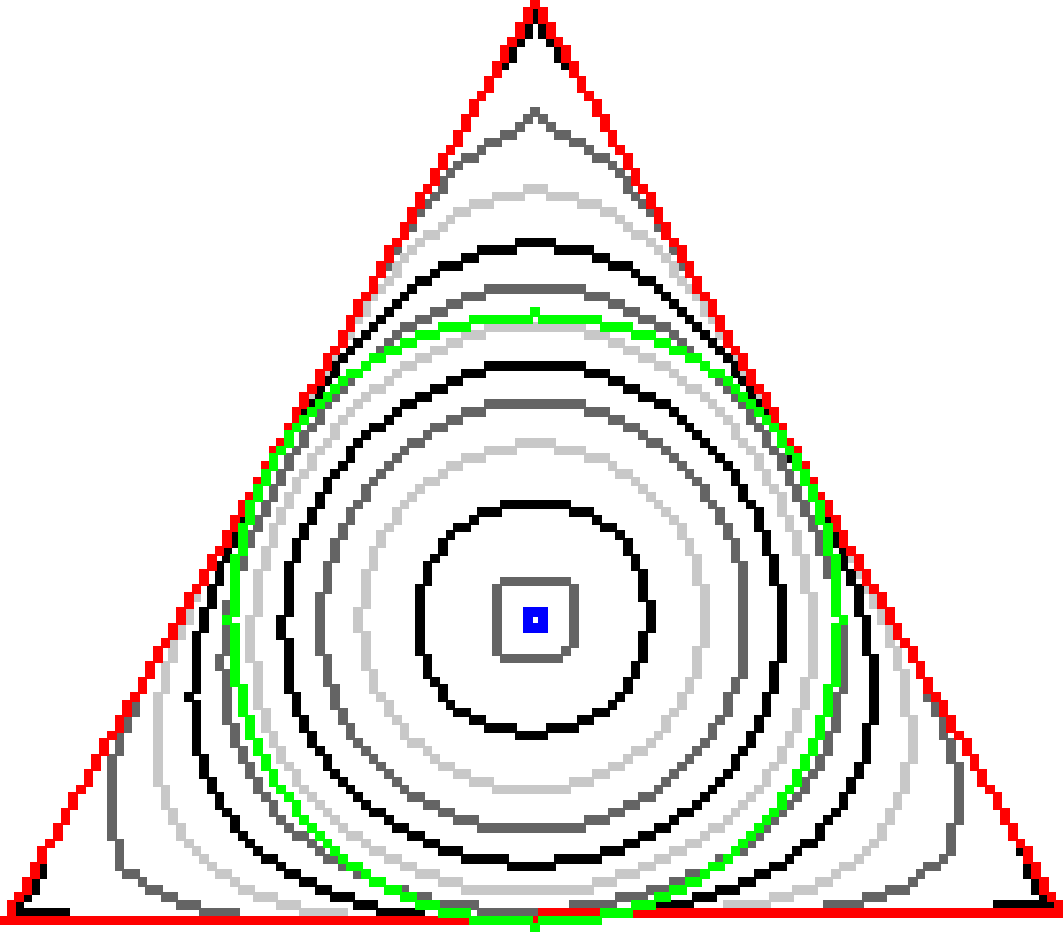
\includegraphics[scale=0.25]{figures/chapter8/graph-flow/triangle/neigh-0/alpha-0.01/summary.pdf} & 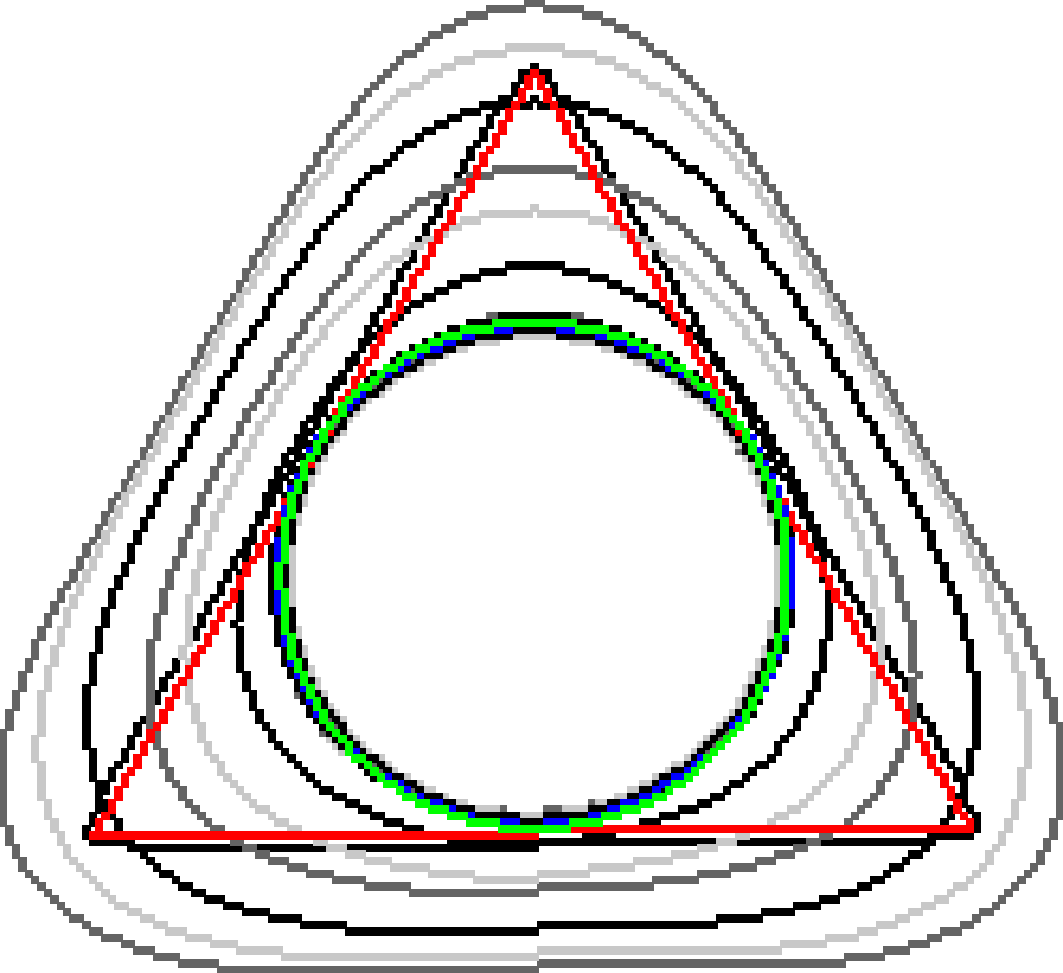
\includegraphics[scale=0.25]{figures/chapter8/graph-flow/triangle/neigh-2/alpha-0.01/summary.pdf} & 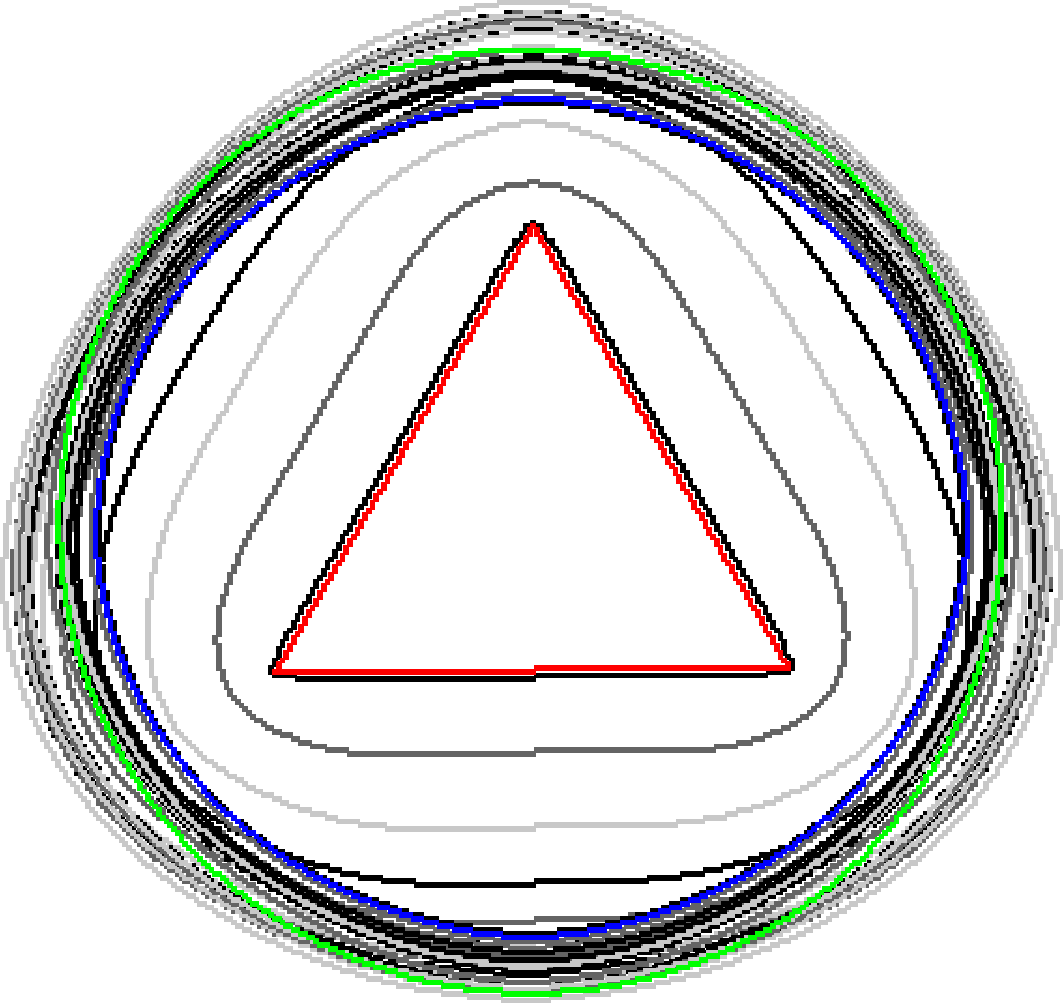
\includegraphics[scale=0.25]{figures/chapter8/graph-flow/triangle/neigh-2/alpha-0.001/summary.pdf}\\
0-GraphFlow & 9-GraphFlow, $\alpha=0.01$ & 9-GraphFlow, $\alpha=0.001$
\end{tabular}}

\subfloat[]{
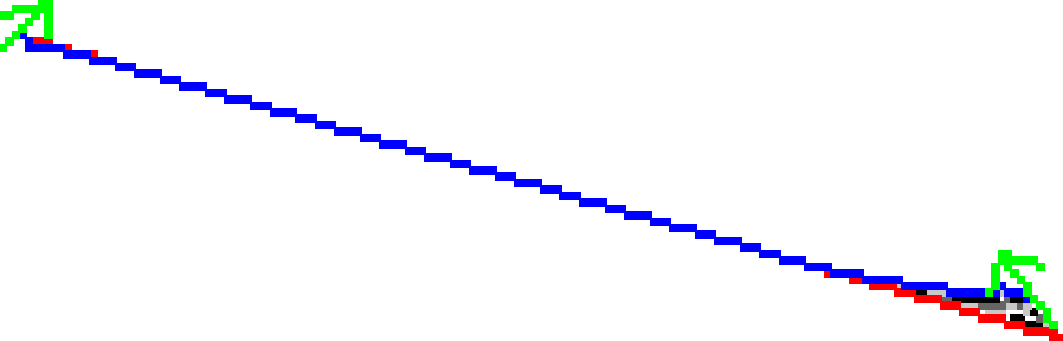
\includegraphics[scale=0.4]{figures/chapter8/constrained-elastica/curve-3/lp-0.001/summary.pdf}
}

\caption{The LSGF algorithm can shrink and grow accordingly with length penalization and it converges to shape closer to the global optimum (green curve) in the free Elastica problem. In the constrained Elastica, we believe that we can improve the results by using a larger, possibly random, neighborhood. We are using $a=2$ and shapes are displayed at every $10$ iterations.}
\label{fig:graph-flow-neigh2-results}
\end{figure}

\section{Injecting data term}

The GrabCut model (see \ref{chapter:appendix-grabcut-model}) is the state-of-art graph-based technique for image segmentation tasks . The GrabCut model possesses two data term components, one related to the boundary, and another to the region. Several works tried to inject geometric information in a graph-cut framework for image segmentation. While some works were sucessfuly in injecting perimeter penalization, those that attempt to include curvature suffered from lack of precision, lack of theoretical guarantees and high running times. In this section we propose a model that advances in these two criterias.

Let $I:\Omega \rightarrow [0,1]^3$ a color image. We define $I(O_m)$ as the subset of $I$ restricted to the optimization region $O_m$. Let $X_m = X(I(O_m))$ and $x$ a possible binary assignment. We recall the GrabCut minimization energy for given parameters $\Lambda=(\lambda_r, \lambda_b)$, image $I$ and labeling $x$.

\begin{align*}
	grabc_{\Lambda}(I,x) &= \lambda_r \sum_{p \in \Omega}{regional(I,x,p)} + \lambda_b \sum_{p,q \in \Omega}{boundary(I,x,p,q)}.
\end{align*}

To construct the graph $G(\mathcal{V},\mathcal{E})$, we define the edge's weight function $w$ such that curvature and data terms are contemplated. Therefore,  

\[
	\forall p,q \in O_m, \quad w(v_p,v_q) = \left\{ \begin{array}{ll}
		\beta(u(S,p) + u(S,q)) + \lambda_b boundary(I,x,p,q), & \text{if } p,q \notin T	\\
		\beta M + \lambda_r regional(I,x,p,q), & \text{if } p \in T \text{ xor } q \in T \\
		0, & \text{otherwise}
	\end{array},\right.
\]

The validation function is defined as

\begin{align*}
val_{(\Theta,\Lambda)}(S^{(k-1)},I,x^{(k-1)}) &= \hat{E}_{\Theta}(S) + grabc_{\Lambda}(I,x)
\end{align*}

Finally, the squared curvature correction algorithm is described as

\begin{algorithm}
 \SetKwData{It}{k}
 \SetKwData{MIt}{maxIt}
 \SetKwData{Delta}{delta}
 \SetKwData{Tol}{tolerance}
 \SetKwInOut{Input}{input}\SetKwInOut{Output}{output}
 \SetKwComment{comment}{//}{}
 
 \Input{A digital set $S$; the optimization band $m$; the neighborhood explorer set size $a$;  parameter vector $\Theta=(\alpha,\beta)$; data term coefficients $\Lambda=(\lambda_r,\lambda_b)$; tolerance $tolerance$.}
 \BlankLine
 $S^{(0)} \longleftarrow S$\;
 $k \longleftarrow 1$\;
 \Delta $\longleftarrow +\infty$\;
 \While{ \It $<$ \MIt \bf{and} \Delta $>$ \Tol  }{ 	
	$candidates \longleftarrow \{\}$\;
	\comment{Candidate selection}
 	\ForEach{ $X \in N_a(S^{(k)})$ }
 	{
 		$candidates \longleftarrow candidates \cup x\big( \; \{ p \; | \; v_p \in C_s( X ) \} \; \big)$\;
 	}

	\comment{Candidate validation}
	$S^{(k)} \longleftarrow \displaystyle \argmin_{x \in candidates}{ val_{(\Theta,\Lambda)}(S^{(k-1)},I,x^{(k-1)})}$\; 	
	\It $\longleftarrow$ \It $+1$\;
	\Delta $\longleftarrow | val_{(\Theta,\Lambda)}(S^{(k)},I,x^{(k)}) - val_{(\Theta,\Lambda)}(S^{(k-1)},I,x^{(k-1)}) |$\;
	
 }
 \caption{LSGF squared curvature segmentation correction algorithm.}
 \label{alg:legc-segmentation-algorithm}  
\end{algorithm}


\begin{figure}
\center
\begin{tabular}{cccc}
\multirow{2}{*}{Seeds} & \multirow{2}{*}{GrabCut} & $\alpha=0.5, \beta=0.0,$ & $\alpha=0.5, \beta=1.0,$\\
& & $\lambda_r=\lambda_b=2.0$ & $\lambda_r=\lambda_b=2.0$\\
 	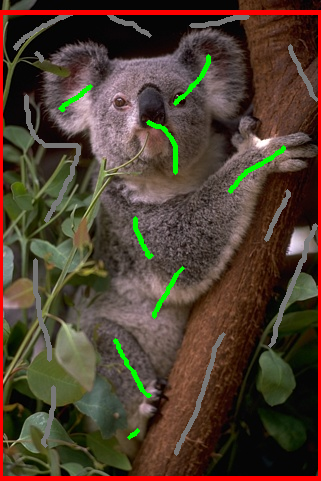
\includegraphics[scale=0.25]{figures/chapter8/segmentation/coala/k-0.0/seeds.png} & 
 	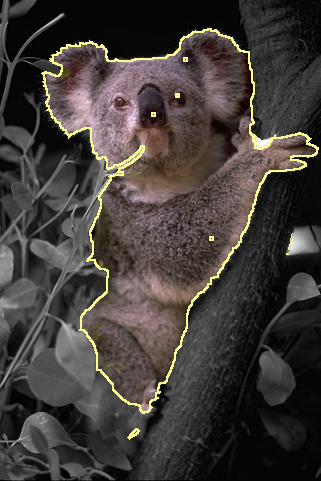
\includegraphics[scale=0.25]{figures/chapter8/segmentation/coala/k-0.0/gc-seg.png} &  	
 	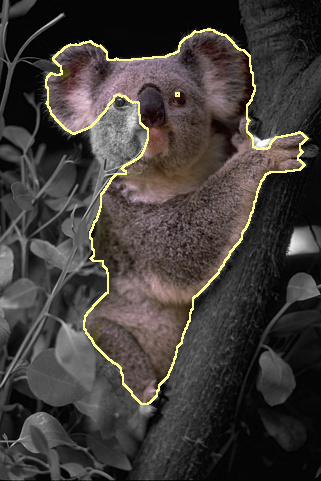
\includegraphics[scale=0.25]{figures/chapter8/segmentation/coala/k-0.0/corrected-seg.png} &  	
 	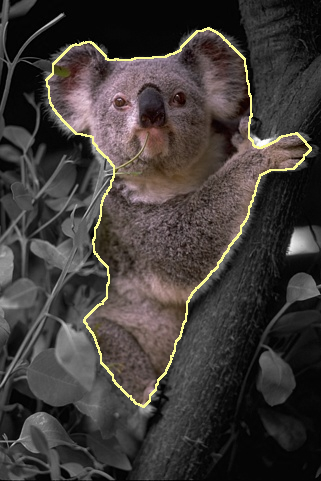
\includegraphics[scale=0.25]{figures/chapter8/segmentation/coala/k-1.0/corrected-seg.png}
\end{tabular}	
\caption{Given foreground (green) and background (gray) seeds at picture (a); GrabCut produces picture (b) which is used as input of the GraphFlow Contour Correction algorithm; in pictures (c) and (d) we display the output of Contour Correction algorithm with and without squared curvature regularization. }
\label{fig:ch8-segmentation}
\end{figure}


\section{A second graph-cut model}
\sketch{Talk about the first graph-cut model attempted at the very beginning.}